\documentclass[12pt]{article}

% Packages
\usepackage[utf8]{inputenc}
\usepackage{amsmath, amssymb}
\usepackage{geometry}
\usepackage{graphicx}
\usepackage{amsfonts}
\usepackage{amsmath}
\usepackage{amssymb}
\usepackage{hyperref}
\usepackage{booktabs}
\geometry{margin=1in}

% Title info
\title{Applied Statistical Methods - Assignment X}
\author{Author Name}
\date{\today}

\begin{document}

% Title
\maketitle

% Header are created like this
\section{Here is a main Header}

This tex-file is as a template for the assignments but also includes some useful information on how to do headings, write equations and insert figures. A useful tip when working in overleaf is to press "compile" quite often so that any potential errors can be found quickly.

% And subheaders like this
\subsection{Here is a subheading}

Lorem Ipsum


\section{Writing equations}

Equations can be written in "math"-mode which puts the equation on a separate line, or just as a part of the regular text. For math mode, use

\begin{equation*}
    Y = \alpha + \beta_0X_1+\beta_1+\varepsilon
\end{equation*}

And for in-line text just write $x=a+b$, but don't do any long equations or formulas in this way, use math-mode instead if so.

The list of Greek letters and mathematical operators is found at \href{https://www.overleaf.com/learn/latex/List_of_Greek_letters_and_math_symbols}{this Overleaf page}.

Sums, products and fractions are written as:

\begin{equation*}
    \sum_{i=1}^{n}
\end{equation*}

\begin{equation*}
    \prod_{i=1}^{n}
\end{equation*}

\begin{equation*}
    \frac{(n-1)S^2}{\sigma^2}
\end{equation*}

The asterix "*" in equation* means that the equation should not be numbered. Without it you get:

\begin{equation}\label{eq:linear_equation}
    Y = \alpha + \beta_0X_1+\beta_1+\varepsilon
\end{equation}

Note that it has a label so it can be referenced (Equation \ref{eq:linear_equation}).

\section{Inserting figures}

First, ensure that the figure is saved in your folder in Overleaf. Then do this

\begin{figure}[ht]
    \centering
    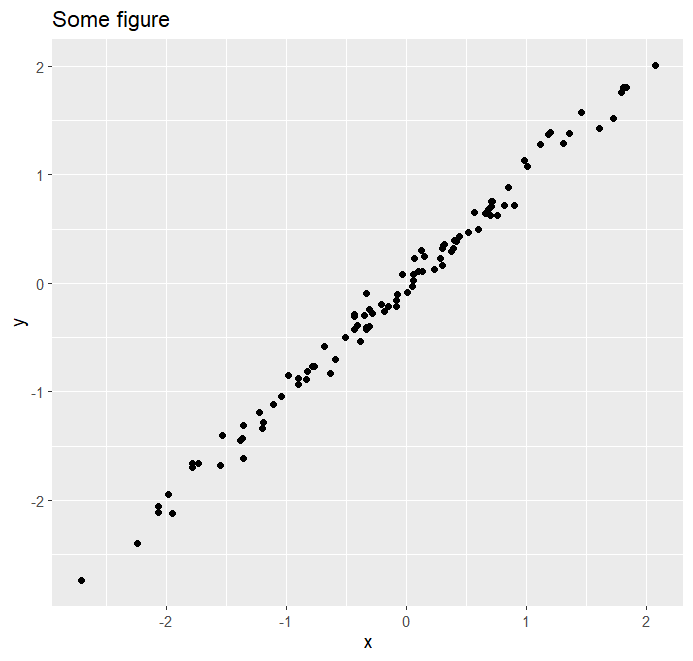
\includegraphics[width=0.6\linewidth]{test_figure.png}
    \caption{Example figure}
    \label{fig:example_figure}
\end{figure}

A figure can be referred to in this way: Figure \ref{fig:example_figure}. The part "ht" in the figure ensures that when compiling to pdf, the figures stays relatively close to where you put in in the text. Some options are found in \href{https://www.overleaf.com/learn/latex/Positioning_images_and_tables}{this Overleaf page}

\section{Making Tables}

If you need to make a table, it can be constructed like in Table \ref{tab:example_table}. "c" in "c|c" means center, and can be changed to "l" or "r" for left or right alignment.

\begin{table}[h]
    \centering
    \begin{tabular}{c|c}
    \toprule
       column1  & column2  \\
       \midrule
        1 & 2 \\
        3  & 4 \\
         5  & 6 \\
    \end{tabular}
    \caption{Example table}
    \label{tab:example_table}
\end{table}

\end{document}
